\section{Results}
L'implémentation des différentes méthodes présentées dans ce rapport est disponible sur \href{https://github.com/ElouanV/mlrf-sciag-2024}{GitHub}, où vous pourrez retrouver davantage de figures ainsi que reproduire les résultats que l'on vous présente ici. Pour les modèles, nous avons utilisé la librairie \href{https://scikit-learn.org/stable/}{Sklearn}

Nous avons ici comparé les trois modèles en utilisant les trois méthodes d'extraction de features sur chaque modèle. Dans un premier temps, nous comparons les résultats avec les hyperparamètres par défaut de \textit{Sklearn} pour comparer les différentes méthodes.
Ensuite, nous étudierons plus en détails chaque méthode avec les modèles qui a le mieux performé pour affiner les hyperparamètres pour chaque méthode d'extraction de feature.

Les modèles que nous présentons ici ont été entraînés sur l'ensemble des données d'entraînement, c'est-à-dire 50 000 instances et les résultats présentés sont les scores obtenus sur l'ensemble de tests de 10 000 instances. Pour la sélection fine des hyperparamètre, nous avons utilisé la \textit{GridSearch} implémenté dans \textit{Sklearn} avec 3 cross-validation.

Nous évaluerons nos modèles en regardant l'accuracy, la courbe ROC ainsi que la matrice de confusion.

\begin{table}[ht]
\centering
\begin{tabular}{|c|c|c|c|}
\toprule
Model & Flatten & Color Histrogram & BoVW \\
\midrule
LogisticRegression& 34.47\% & 23.01\%&\textbf{20.41\%} \\
KNN & 34.15\%& 22.68\%& 13.34\% \\
RandomForest & \textbf{47.01\%} & \textbf{26.61\%} & 18.26\% \\
\bottomrule
\end{tabular}
\caption{Accuracy de chaque modèle sur chaque méthode d'extraction sans affinage des hyperparamètres sur le jeu de donnée CIFAR-10}
\label{tab:result_no_ft}
\end{table}
Le tableau \ref{tab:result_no_ft} présente l'accuracy de chaque modèle sur chaque méthode d'extraction sans affinage des hyperparamètres. La première chose qui saute aux yeux est le fait que la méthode d'extraction de feature le plus élaboré, \textit{BoVW}, produit les résultats les moins intéressants. On observe un accuracy deux fois plus élevée avec le meilleur utilisant l'image aplatie par rapport au meilleur modèle utilisant \textbf{BoVW}. Sur \textit{BoVW}, la régression logistique semble obtenir les meilleurs résultats.
D'autre part, le KNN semble ne pas bien marcher sur ce problème, comme nous pouvions l'espérer, car il n'est pas adapté à ce genre de tâche.
En revanche, le modèle random forest obtient les meilleurs résultats sur l'image aplatie (26.61\%) et l'histogramme de couleur (47.01\%).
La figure \ref{fig:confusion} montre les matrices de confusion des meilleurs modèles. La matrice de confusion du random forest sur image aplatie est évidemment plus propre, mais on remarque aussi que la random forest sur l'histogramme de couleur arrive à bien classifier les avions et bateau, et lorsqu'il y a une erreur, ils sont confondu l'un et l'autre. Cela vient probablement du fait qu'ils partagent des caractéristiques communes: souvent l'objet en blanc sur un fond bleu, qui est singulier par rapport aux images de chat, de chien etc. où l'on retrouve un fond vert avec un objet marron.
\begin{figure}
\centering
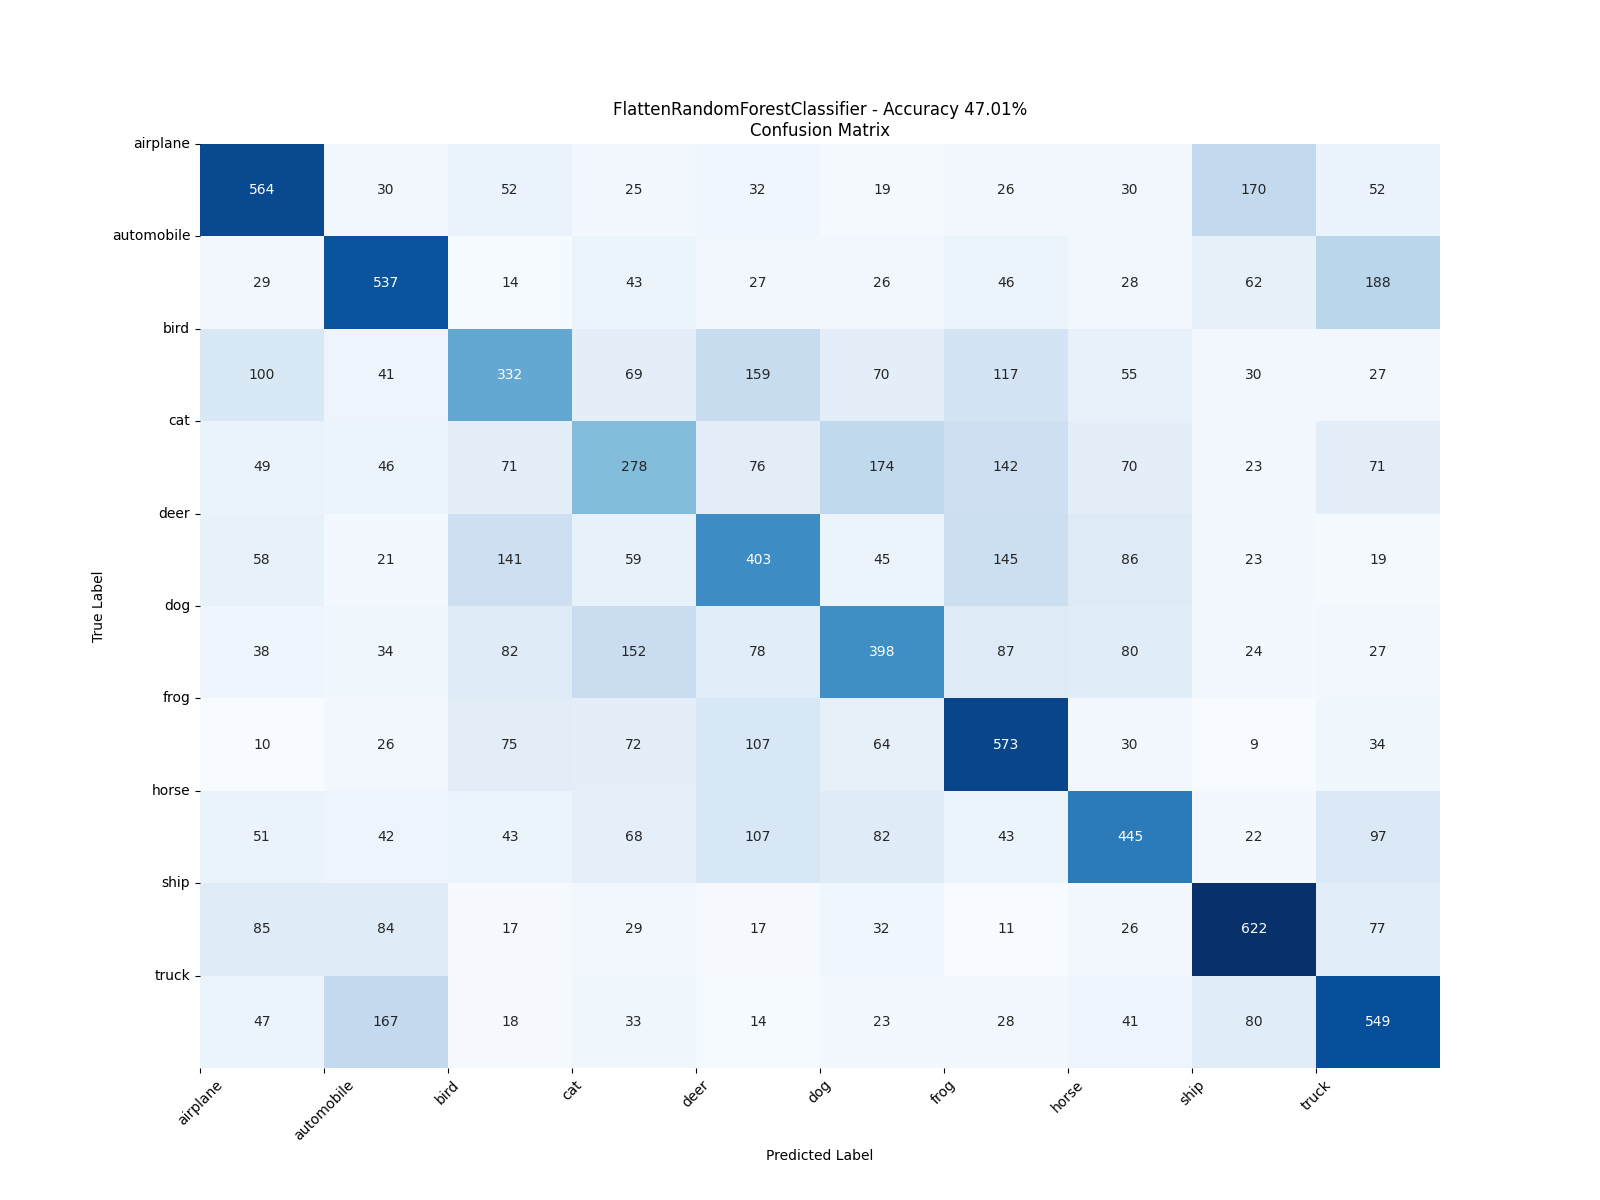
\includegraphics[scale=0.2]{figures/confusion_matrix_RandomForestClassifier_flatten.png}
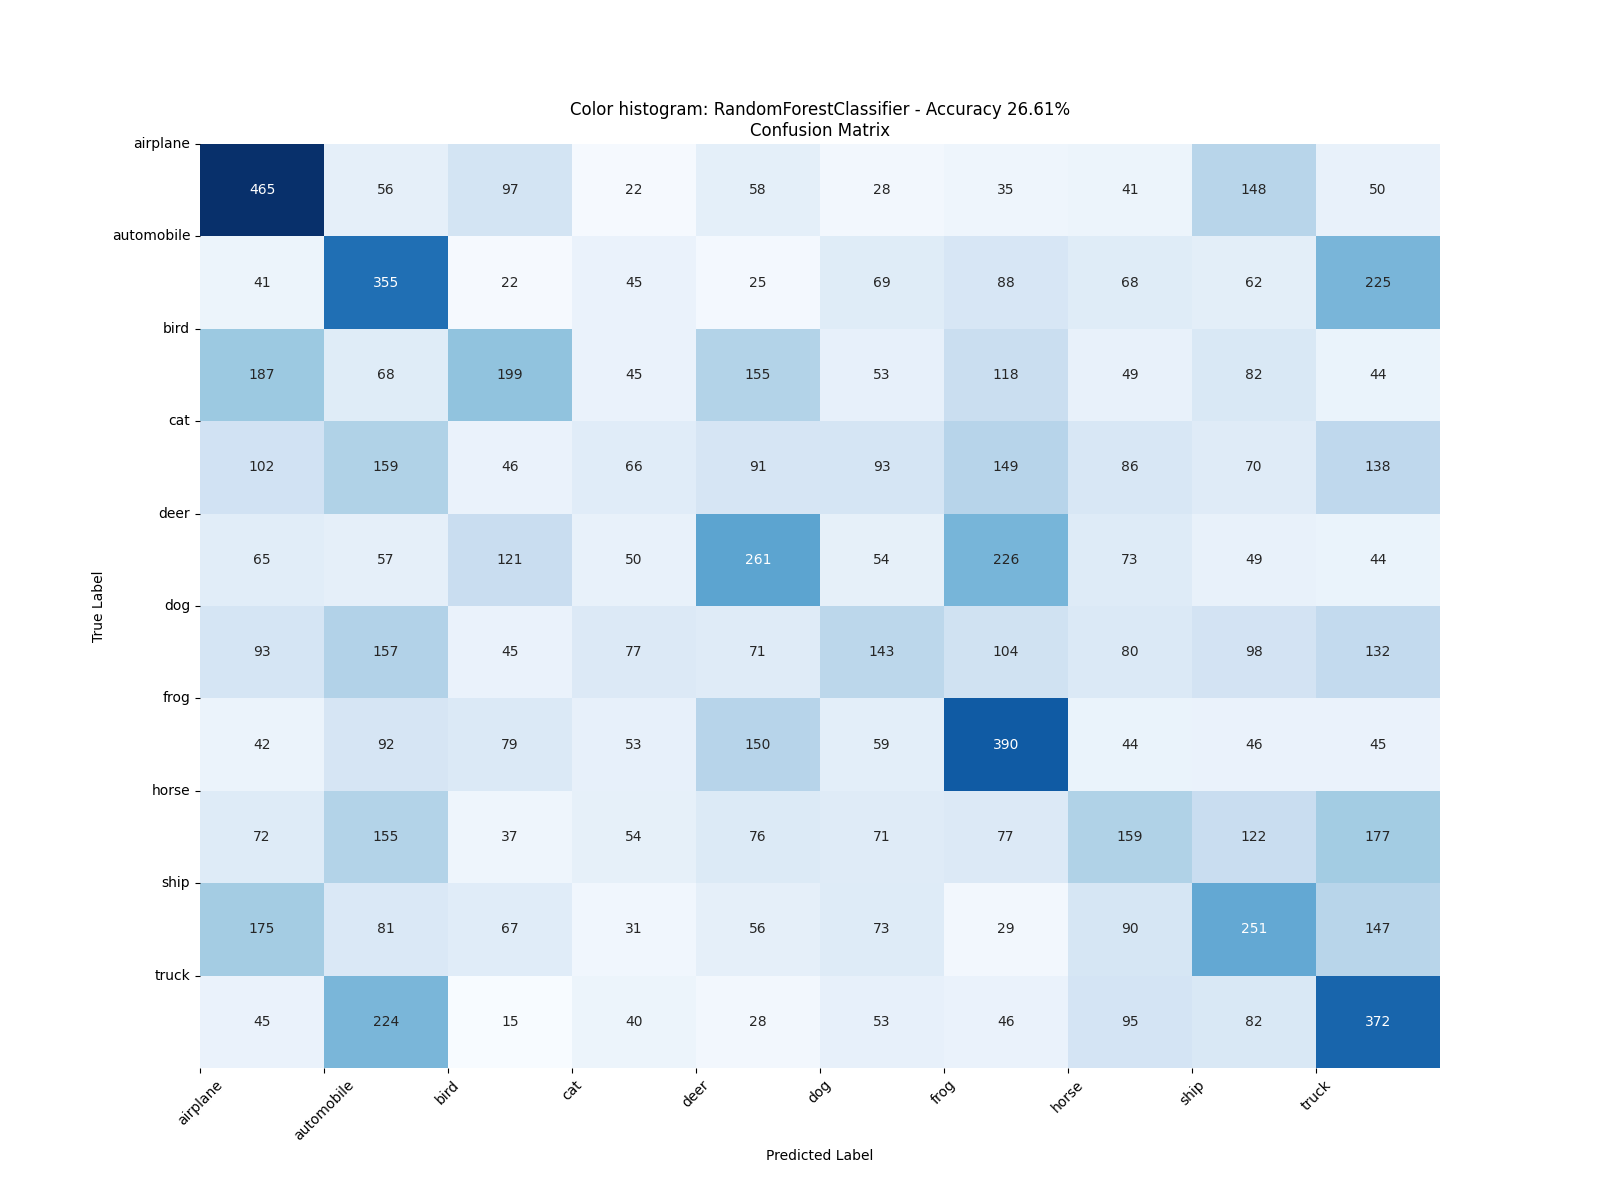
\includegraphics[scale=0.2]{figures/confusion_matrix_RandomForestClassifier_color.png}
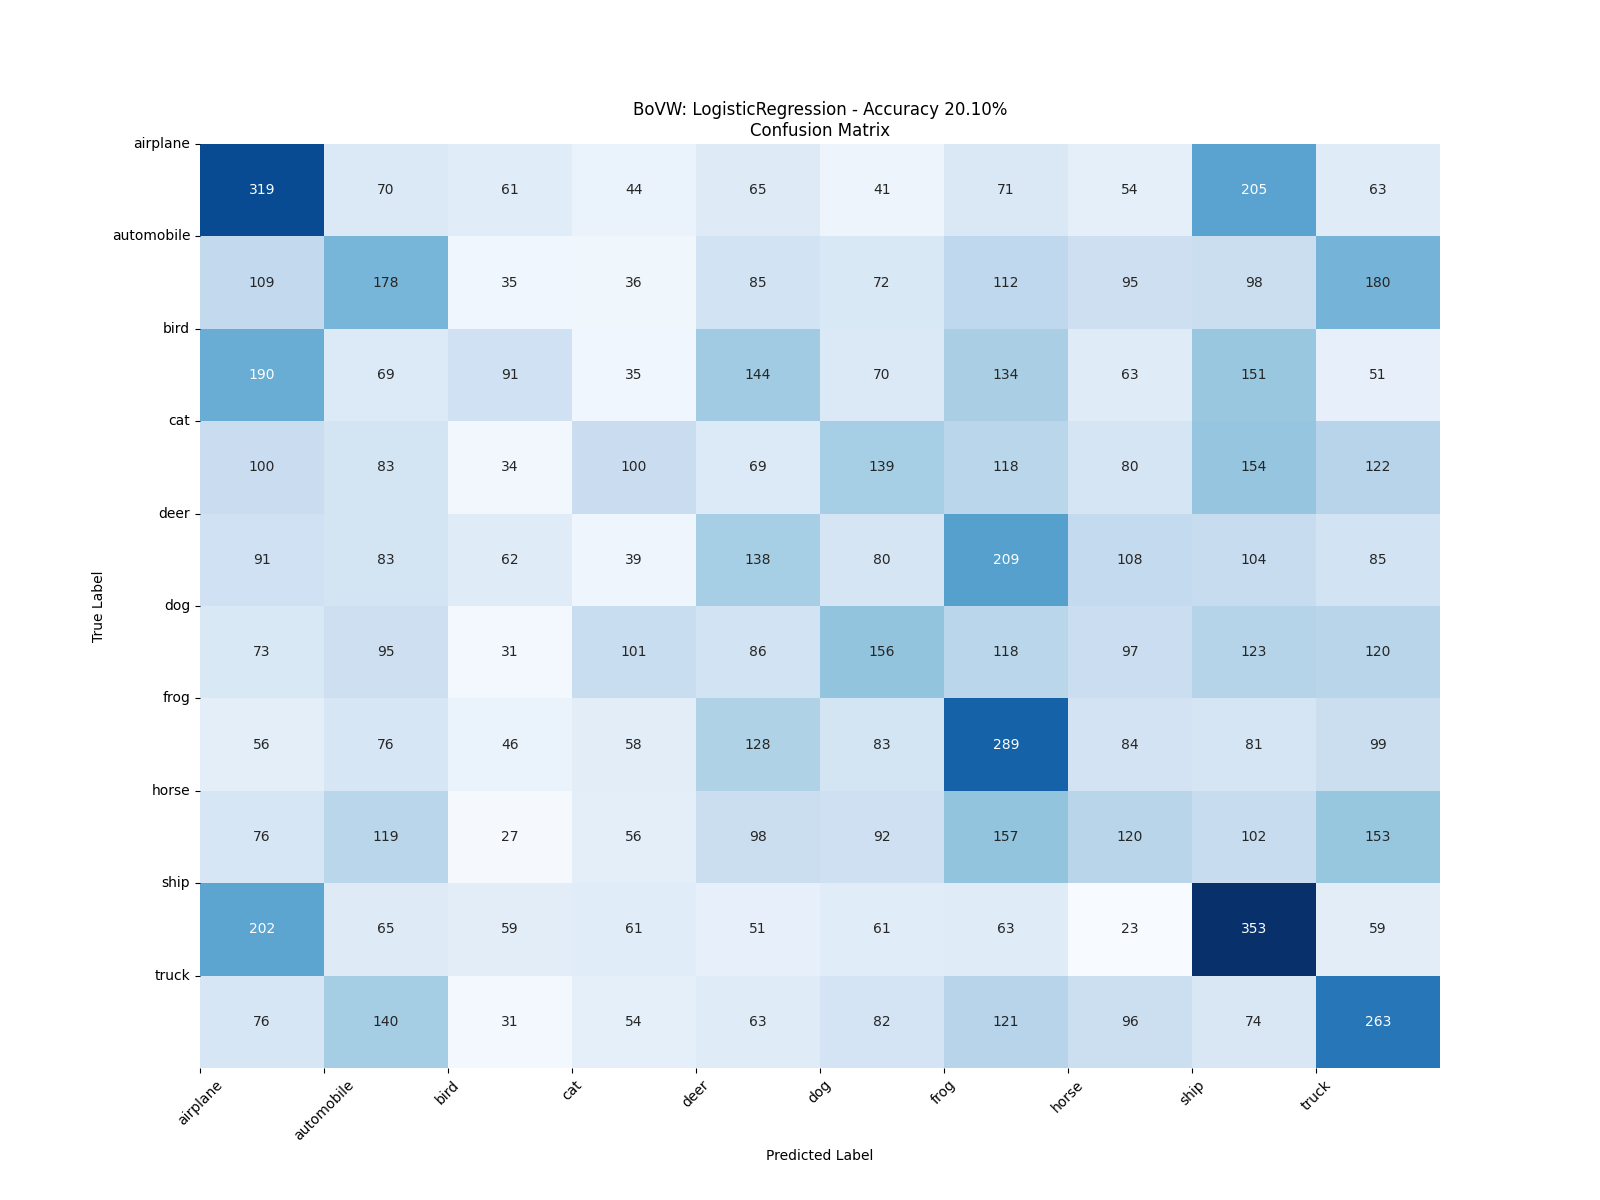
\includegraphics[scale=0.2]{figures/confusion_matrix_LogisticRegression_bovw_ft.png}
\caption{Matrice de confusion pour les meilleurs modèles selon la méthode d'extraction de features: Random forest sur image applatie (haut gauche), random forest sur histogramme de couleur (haut droite) et regression logistique sur \textit{BoVW} (bas)}
\label{fig:confusion}
\end{figure}

Maintenant, nous allons affiner les hyperparamètres pour le random forest sur l'image aplatie et l'histogramme de couleur et la régression logistique sur le \textit{BoVW} pour voir si cela peut améliorer les résultats de la classification. La Figure \ref{tab:fine_tuning} présente l'évolution de l'accuracy avec et sans affinage des hyperparamètres.

\begin{table}[ht]
\centering
\begin{tabular}{|c|c|c|c|}
\toprule
& RandomForest + Flatten & RandomForest + ColorHist & LogisticRegression + BoVW \\
\midrule
Sans fine-tuning & 47.01\% & 26.61\% & 20.41\% \\
Avec fine-tuning & 48.53\% & 27.98\% & 20.41\% \\
\bottomrule
\end{tabular}
\caption{Evolution de l'accuracy après affinage des hyperparamètres pour une régression logistique avec BoVW, et deux random forest avec image aplatie et histogramme de couleur.}
\label{tab:fine_tuning}
\end{table}
La régression logistique avec \textit{BoVW} ne progresse pas en affinant ses hyperapamètres, il semblerait que les paramètres par défauts produisent déjà les meilleurs résultats.
Pour les modèles sur utilisant les random forest, les résultats s'améliorent de manière intéressante, on atteint $48.53\%$ d'accuracy avec l'image aplatie.

Bien que les résultats présentés ici soient intéressants, nous n'avons pas utilisé d'apprentissage profond. Si on souhaite se comparer à l'état de l'art, \cite{kabir2023reduction} présente $99.70\%$ d'accuracy sur ce dataset utilisant les transformers. Nos résultats sont ridicules si on les compare simplement comme ça, mais il ne faut pas oublier que la méthode qui obtient le meilleur résultat ici est celle qui ne requiert strictement aucun pré-traitement des images, qui est donc légère. En limitant le nombre d'arbres dans le random forest, le modèle aussi peut être relativement léger, plus qu'un transformer en tout cas.